\documentclass{beamer}

\mode<presentation> {

\usetheme{Montpellier}
\usecolortheme{beaver}

%\setbeamertemplate{footline} % To remove the footer line in all slides uncomment this line
%\setbeamertemplate{footline}[page number] % To replace the footer line in all slides with a simple slide count uncomment this line

%\setbeamertemplate{navigation symbols}{} % To remove the navigation symbols from the bottom of all slides uncomment this line
}

\usepackage{graphicx} % Allows including images
\usepackage{booktabs} % Allows the use of \toprule, \midrule and \bottomrule in tables
\usepackage{listings}
\usepackage{tikz}
\usepackage{multicol}
\usepackage{color}
\setlength{\columnsep}{2cm}

%------------------------------------------------------------------------------
% TITLE PAGE
%------------------------------------------------------------------------------

\title[Intro to \LaTeX]{Introduction to \LaTeX}

\author{Scarlet \& Jeremy}
\institute[Cornell University]{
Cornell University \\
\medskip
\textit{hy323 \& jlf248}
}
\date{\today}


\usetikzlibrary[topaths]
\newcount\mycount

\begin{document}

\begin{frame}
  \titlepage
\end{frame}

\begin{frame}
  \frametitle{Overview}
  \tableofcontents
\end{frame}

\begin{frame}
  \frametitle{What is \LaTeX?}
  \begin{itemize}
    \item A document preparation and markup language for high-quality typesetting
      \begin{itemize}
        \item i.e. it takes your confusing looking markup and compiles it to a beautiful PDF
      \end{itemize}
    \item Widely used in academic research, especially the sciences
      \begin{itemize}
        \item i.e. it gives off a very professional feel, even when what you're writing makes no sense $\ddot\smile$
      \end{itemize}
  \end{itemize}
\end{frame}

%------------------------------------------------------------------------------
\section{Basic}
%------------------------------------------------------------------------------

\subsection{Setting Up}
\begin{frame}[fragile]
  \frametitle{Setting Up \& Compiling}
    \begin{itemize}
      \item Windows: use cygwin
      \item Mac: https://tug.org/mactex/
        \begin{itemize}
          \item The instructions are really good
          \item The files you have to download/install are huge (on the order of GBs)
        \end{itemize}
      \item I highly recommend using an editor like TeXshop, TeXworks, Vim, Emacs, or even Sublime Text to write LaTeX with because they all are either built to compile your documents or have well supported plugins that do it all for you.
    \end{itemize}
\end{frame}
\begin{frame}[fragile]
  \frametitle{Basic Document Structure}
    \begin{itemize}
      \item \verb.\documentclass[options]{article}.
      \item Preamble -- import external packages, set up page formatting, define your own macros, etc.
      \item \verb.\begin{document}.
      \item Some sort of title
      \item \verb.\section{Section Title}.
      \item Some content
      \item \verb.\subsection{Subsection Title}.
      \item More content
      \item etc. etc. etc.
      \item \verb.\end{document}.
    \end{itemize}
\end{frame}


\subsection{Basic Writing}
\begin{frame}[fragile]
  \frametitle{Text Paragraphs}
  \begin{itemize}
    \item Any time LaTeX sees a blank line, it treats the next line as
      the start of a new paragraph
    \item You can force new lines with \verb.\\.
    \item Add indentation by \verb.indent. or suppress it with \verb.\noindent.
  \end{itemize}
  \begin{verbatim}
    This is the start of a new paragraph.
    This is not, even though I'm on a new line.

    This is another paragraph. \\
    Now I've forced it onto a new line, but not a new
    paragraph.
  \end{verbatim}
\end{frame}
\begin{frame}[fragile]
  \frametitle{Text Style}
  \begin{itemize}
    \item There are all the normal text styles you'd expect from a word processor, but for some you have to use external packages.
    \item For example, to use color you need to add \verb.\usepackage{color}. to your preamble
  \end{itemize}
  \begin{tabular}{ll}
    \verb.\textbf{Hello World}. & \textbf{Hello World} \\
    \verb.\emph{Hello World}. & \emph{Hello World} \\
    \verb.\textsc{Hello World}. & \textsc{Hello World} \\
    \verb.\texttt{Hello World}. & \texttt{Hello World} \\
    \verb.\underline{Hello World}. & \underline{Hello World} \\
    \verb.\textcolor{red}{Hello World}. & \textcolor{red}{Hello World} \\
  \end{tabular}
\end{frame}
\begin{frame}[fragile]
  \frametitle{Titles}
  \begin{itemize}
    \item There are some shortcuts for you to make nice titles, but you don't \emph{have} to use them
    \item A title will typically look like
  \end{itemize}
  \begin{verbatim}
    \title{This is a Title}
    \author{Scarlet \& Jeremy}
    \date{November 2014}
    \maketitle
  \end{verbatim}
\end{frame}
\begin{frame}[fragile]
  \frametitle{Sections}
  \begin{itemize}
    \item There are some shortcuts for you to make nice section headings (think chapters in a book, questions on a problem set, etc.)
    \item Sections will typically look like
  \end{itemize}
  \begin{verbatim}
    \section{A big section title}
    \subsection{A nested section title}
    \subsubsection{An even more nested title}
  \end{verbatim}
\end{frame}
\begin{frame}[fragile]
  \frametitle{Text Size}
  \begin{itemize}
    \item There are built in commands for changing text size
    \item You can use them with \verb.\textsize{your text}.
    \item Here are some examples
  \end{itemize}
  \begin{tabular}{ll}
    \verb.\tiny. & \tiny{tiny text} \\
    \verb.\scriptsize. & \scriptsize{scriptsize text} \\
    \verb.\footnotesize. & \footnotesize{footnotesize text} \\
    \verb.\small. & \small{small text} \\
    \verb.\normalsize. & \normalsize{normalsize text} \\
    \verb.\large. & \large{large text} \\
    \verb.\Large. & \Large{Large text} \\
    \verb.\LARGE. & \LARGE{LARGE text} \\
    \verb.\huge. & \huge{huge text} \\
    \verb.\Huge. & \Huge{Huge text} \\
  \end{tabular}
\end{frame}

\subsection{List Structures}
\begin{frame}[fragile]
\frametitle{Enumerate} %done
  \begin{multicols}{2}
    \begin{verbatim}
        \begin{enumerate}
            \item one.
            \item two.
        \end{enumerate}
    \end{verbatim}
  \columnbreak
    \begin{enumerate}
      \item one.
        \item two.
    \end{enumerate}
  \end{multicols}

  \begin{multicols}{2}
    \begin{verbatim}
        \begin{enumerate}[a)]
            \item one.
            \item two.
        \end{enumerate}
    \end{verbatim}
  \columnbreak
    \begin{enumerate}[a)]
      \item one.
        \item two.
    \end{enumerate}
  \end{multicols}
\end{frame}

\begin{frame}[fragile]
\frametitle{Itemize} %done
  \begin{multicols}{2}
    \begin{verbatim}
      \begin{itemize}
        \item one.
        \item two.
      \end{itemize}
    \end{verbatim}
    \columnbreak
    \begin{itemize}
      \item one.
      \item two.
    \end{itemize}
  \end{multicols}

  \begin{multicols}{2}
    \begin{verbatim}
      \begin{itemize}
        \item[Item1] one.
        \item[Item2] two.
      \end{itemize}
    \end{verbatim}
    \columnbreak
      \begin{itemize}
        \item[Item1] one.
        \item[Item2] two.
      \end{itemize}
  \end{multicols}
\end{frame}

\begin{frame}[fragile]
\frametitle{Nested Lists} %done
  \begin{multicols}{2}
    \begin{verbatim}
      \begin{enumerate}
        \item enumerate1
          \begin{itemize}
            \item item1
            \item item2
          \end{itemize}
        \item enumerate2
      \end{enumerate}
    \end{verbatim}
    \columnbreak
      \begin{enumerate}
        \item enumerate1
          \begin{itemize}
            \item item1
            \item item2
          \end{itemize}
        \item enumerate2
      \end{enumerate}
  \end{multicols}
\end{frame}

\subsection{Math Mode \& Symbols}
\begin{frame}[fragile]
\frametitle{Math Mode}
  \begin{itemize}
    \item Enter math mode using \$ around texts
  \end{itemize}
  \begin{multicols}{2}
    \begin{verbatim}
      $ math mode $
    \end{verbatim}
    \columnbreak
    $math mode$
  \end{multicols}

  \begin{itemize}
    \item Close \$ to go back to text mode
  \end{itemize}
  \begin{multicols}{2}
    \begin{verbatim}
      $math$ text $math$
    \end{verbatim}
    \columnbreak
    $math$ text $math$
  \end{multicols}

  \begin{itemize}
    \item Or use \verb+\text+ to temporarily go into text mode
  \end{itemize}
  \begin{multicols}{2}
    \begin{verbatim}
      $math \text{ text } math$
    \end{verbatim}
    \columnbreak
    $math \text{ text } math$
  \end{multicols}
\end{frame}

\begin{frame}[fragile]
\frametitle{Commonly used symbols}
  \begin{multicols}{2}
    \verb+\geq \leq \neq+ \\
    \verb+\oplus \times+ \\
    \verb+\cup \cap+ \\
    \verb+\vee \wedge+ \\
    \verb+\forall \exists \in+  \\
    \verb+\because \therefore+  \\
    \verb+\rightarrow \leftarrow+\\
    \verb+\Rightarrow \Leftarrow+ \\
    \verb+\equiv \approx \sim+ \\
    \verb+\LaTeX+ \\
  \columnbreak
    $\geq$ $\leq$ $\neq$\\
    $\oplus$ $\times$\\
    $\cup$ $\cap$\\
    $\vee$ $\wedge$\\
    $\forall$ $\exists$ $\in$\\
    $\because$ $\therefore$\\
    $\rightarrow$ $\leftarrow$\\
    $\Rightarrow$ $\Leftarrow$\\
    $\equiv$ $\approx$ $\sim $\\
    \LaTeX
  \end{multicols}
  \begin{itemize}
    \item \verb.{ } _ ^ # & $ % ~. Needs to be escaped to be used in text mode.
    \item Use \url{http://detexify.kirelabs.org/classify.html}
  \end{itemize}
\end{frame}

\begin{frame}[fragile]
  \frametitle{Powers and Subscripts}
  \begin{itemize}
    \item Powers, subscripts, fractions are written in math mode!
  \end{itemize}
  \begin{multicols}{2}
    \verb+a^b  a^{multichar}+\\
    \verb+a_b  a_{multichar}+\\
    \verb+\frac{a}{b}+\\
  \columnbreak
    $a^b$ $a^{multichar}$\\
    $a_b$ $a_{multichar}$\\
    $\frac{a}{b}$
  \end{multicols}
\end{frame}

\subsection{Math Paragraphs \& Alignment}
\begin{frame}[fragile]
  \frametitle{Math Paragraphs}
  \begin{itemize}
    \item simple line of math can be written in \verb+\[ ... \]+
    \item Automatically in math mode
  \end{itemize}
  \begin{verbatim}
  \[
    \{(pk,sk) \leftarrow Gen(1^n) :
      (pk,Enc_{pk} (m_0))\}_n
  \]
  \end{verbatim}
  \[
    \{(pk,sk) \leftarrow Gen(1^n) : (pk,Enc_{pk} (m_0))\}_n
  \]
  \begin{itemize}
    \item But you can't linebreak!
  \end{itemize}
\end{frame}

\begin{frame}[fragile]
  \frametitle{Alignment}
  \begin{itemize}
    \item Automatically in math mode
    \item \verb.align. has equation numbers by default, \verb.align*. doesn't
  \end{itemize}
  \begin{multicols}{2}
    \begin{verbatim}
      \begin{align}
        f(x) = 5x^2 + 4x + 3\\
        g(x) = 6x + 7
      \end{align}
    \end{verbatim}
  \columnbreak
    \begin{align}
      f(x) = 5x^2 + 4x + 3\\
      g(x) = 6x + 7
    \end{align}
  \end{multicols}

  \begin{multicols}{2}
    \begin{verbatim}
      \begin{align*}
        f(x) = 5x^2 + 4x + 3\\
        g(x) = 6x + 7
      \end{align*}
    \end{verbatim}
  \columnbreak
    \begin{align*}
      f(x) = 5x^2 + 4x + 3\\
      g(x) = 6x + 7
    \end{align*}
  \end{multicols}
\end{frame}

\begin{frame}[fragile]
  \frametitle{Alignment}
  \begin{itemize}
    \item Align equations using anchors \&
    \item Can be followed by anything, not just =
  \end{itemize}
  \begin{multicols}{2}
    \begin{verbatim}
      \begin{align*}
        f(x) &= (x + 2) - 2 \\
             &= x \\
             &\rightarrow wow!
      \end{align*}
    \end{verbatim}
  \columnbreak
    \begin{align*}
      f(x) &= (x + 2) - 2\\
           &= x \\
           &\rightarrow wow!
    \end{align*}
  \end{multicols}
\end{frame}

\begin{frame}[fragile]
  \frametitle{More Alignment}
  \begin{itemize}
    \item LaTeX assumes that each equation consists of two parts separated by
      anchor \&
  \end{itemize}
  \begin{verbatim}
    \begin{align*}
      x&=y           &  w &=z              &  a&=b+c\\
      2x&=-y         &  3w&=\frac{1}{2}z   &  a&=b\\
      -4 + 5x&=2+y   &  w+2&=-1+w          &  ab&=cb
    \end{align*}
  \end{verbatim}
  \begin{align*}
    x&=y           &  w &=z              &  a&=b+c\\
    2x&=-y         &  3w&=\frac{1}{2}z   &  a&=b\\
    -4 + 5x&=2+y   &  w+2&=-1+w          &  ab&=cb
  \end{align*}
\end{frame}

\subsection{Multicols}
\begin{frame}[fragile]
  \frametitle{Multicols}
  \begin{verbatim}
    \begin{multicols}{2}
      \begin{enumerate} % chunk1
        \item A-one
        \item A-two
      \end{enumerate}
      \begin{enumerate} % chunk2
        \item B-one
        \item B-two
      \end{enumerate}
    \end{multicols}
  \end{verbatim}

  \begin{multicols}{2}
  \begin{enumerate}
    \item A-one
    \item A-two
  \end{enumerate}
  \begin{enumerate}
    \item B-one
    \item B-two
  \end{enumerate}
  \end{multicols}
\end{frame}

\begin{frame}[fragile]
  \frametitle{Multicols}
  \begin{verbatim}
    \begin{multicols}{2}
      Latex is beautiful! It is easy to learn!
    \columnbreak        % forces column break
      Computer Science is great!
      Hope this session is helping!
    \end{multicols}
  \end{verbatim}

  \begin{multicols}{2}
    Latex is beautiful! It is easy to learn!
  \columnbreak        % forces column break
    Computer Science is great!
    Hope this session is helping!
  \end{multicols}
\end{frame}

%----------------------------------------------------------------------------------------
\section{Intermediate}
%----------------------------------------------------------------------------------------

\subsection{Defining \& Renewing Commands}
\begin{frame}[fragile]
  \frametitle{New Commands}
  \begin{itemize}
    \item Define environments using \verb.\newcommand{\your_command_name}{what it does}.
    \item Here's an example:
  \end{itemize}
  \begin{verbatim}
    \newcommand{\scarlet}[1][Jeremy]
      {$S_cA^rL_eT$ and {#1}}
  \end{verbatim}
  \newcommand{\scarlet}[1][Jeremy]{$S_cA^rL_eT$ and {#1}}
  \begin{itemize}
    \item Now you can use \verb.\scarlet. in your document to produce this: \scarlet.
    \item Or you can use \verb.\scarlet[Scarlet]. to produce this: \scarlet[Scarlet].
  \end{itemize}
\end{frame}
\begin{frame}[fragile]
  \frametitle{New Environments}
  \begin{itemize}
    \item An environment is anything you use with \verb.\begin{env} contents \end{env}..
    \item Define new environments using \verb.\newenvironment{name}[num]{before}{after}.
    \item Here's an example:
  \end{itemize}
  \begin{verbatim}
    \newenvironment{newitemize}
      {Here goes nothing! \begin{itemize}}
      {\end{itemize} And so ends the list!}
  \end{verbatim}
  \newenvironment{newitemize}
    {Here goes nothing! \begin{itemize}}
    {\end{itemize} And so ends the list!}
  \begin{itemize}
    \item Now you can use it in your document to produce this:
      \begin{newitemize}
        \item item 1
        \item item 2
      \end{newitemize}
  \end{itemize}

\end{frame}
\begin{frame}[fragile]
  \frametitle{Renewing Commands}
  We can also overwrite existing commands (or ones that we made) using \verb.\renewcommand. with the same syntax as \verb.\newcommand.

  A common example would be redefining how sections and subsections look using the following
  \begin{verbatim}
    \renewcommand{\thesection}
      {\Large Exercise \arabic{section}.}
    \renewcommand{\thesubsection}
      {\normalsize (\alph{subsection})}
  \end{verbatim}
  This will give you {\Large Exercise 1} as the section titles and {\normalsize (a)} for the subsections.
\end{frame}

\subsection{Boxes \& Resizing}
\begin{frame}
  \frametitle{Boxes \& Resizing}
\end{frame}

\subsection{Tables, Graphs, \& Figures}
\begin{frame}[fragile]
  \frametitle{Tables}
  \begin{itemize}
    \item Most of the time you won't want to do this by hand
    \item There are lots of online tools that make it easier
      \begin{itemize}
        \item http://truben.no/table/
        \item http://www.tablesgenerator.com/
      \end{itemize}
    \item The basic gist is
  \end{itemize}

  \begin{multicols}{2}
    \begin{verbatim}
      \begin{table}
        \begin{tabular}{|l|r}
        h1   & h2   \\ \hline
        blah & blah \\
        blah & blah \\
        \end{tabular}
      \end{table}
    \end{verbatim}
    \columnbreak
    \begin{table}
      \begin{tabular}{|l|r}
      h1   & h2   \\ \hline
      blah & blah \\
      blah & blah \\
      \end{tabular}
    \end{table}
  \end{multicols}
\end{frame}
\begin{frame}[fragile]
  \frametitle{Tables}
  \begin{itemize}
    \item The \verb.{|l|r}. after \verb.\begin{tabular}. specifies the alignment of each column. \verb.{|l|r}. means the first column should be left aligned and the second column should be right aligned. The other option is using \verb.c. for center alignment.
    \item We can put lines between columns by adding \verb.|.. For example, this \verb.{|c|c|c|}. will add lines around every column.
    \item The \verb.&. separate the items in a row.
    \item We can add lines between rows by using \verb.\\ \hline. instead of just \verb.\\..
  \end{itemize}
\end{frame}
\begin{frame}[fragile]
  \frametitle{Graphs}
  \begin{itemize}
    \item For simple state machines/graphs, I recommend trying out this tool before jumping into the heavyweight stuff: http://madebyevan.com/fsm/.
    \item If that doesn't work, then use \verb.tikz. by declaring \verb.\usepackage{tikz}. in your preamble. And look up examples that are similar to what you want to do on http://www.texample.net/tikz/examples/.
    \item Some people get pretty crazy...
  \end{itemize}
\end{frame}
\begin{frame}[fragile]
  \frametitle{Graphs}
  \centering
  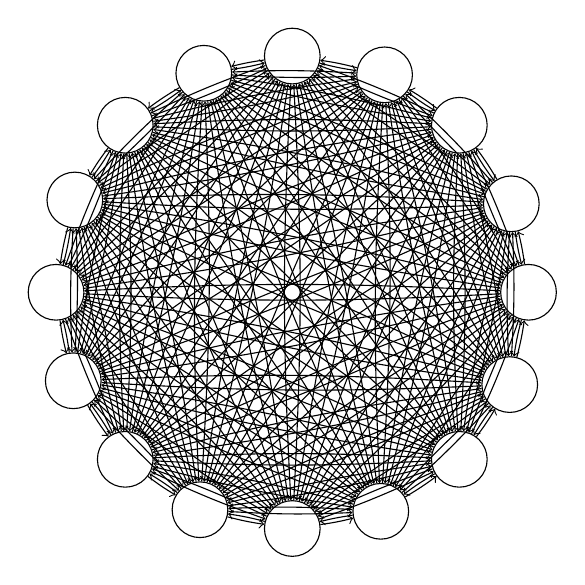
\begin{tikzpicture}[transform shape]
    %the multiplication with floats is not possible. Thus I split the loop in two.
    \foreach \number in {1,...,8}{
        % Computer angle:
          \mycount=\number
          \advance\mycount by -1
    \multiply\mycount by 45
          \advance\mycount by 0
        \node[draw,circle,inner sep=0.25cm] (N-\number) at (\the\mycount:3cm) {};
      }
    \foreach \number in {9,...,16}{
        % Computer angle:
          \mycount=\number
          \advance\mycount by -1
    \multiply\mycount by 45
          \advance\mycount by 22.5
        \node[draw,circle,inner sep=0.25cm] (N-\number) at (\the\mycount:3cm) {};
      }
    \foreach \number in {1,...,15}{
          \mycount=\number
          \advance\mycount by 1
    \foreach \numbera in {\the\mycount,...,16}{
      \path (N-\number) edge[->,bend right=3] (N-\numbera)  edge[<-,bend
        left=3] (N-\numbera);
    }
  }
  \end{tikzpicture}
\end{frame}
\begin{frame}[fragile]
  \frametitle{Figures \& Graphics}
  \begin{itemize}
    \item Include the \verb.graphicsx. package using \verb.\usepackage{graphicsx}. in your preamble.
    \item Here's an example
  \end{itemize}
  \begin{verbatim}
    \begin{figure}[h]
      
\includegraphics[width=0.3\textwidth]
        {./awesomesauce.jpg}
      \caption{This is an amazing picture}
    \end{figure}
  \end{verbatim}
  \begin{figure}[ht]
    \centering
    \label{awesomesauce}
    
\includegraphics[width=0.3\textwidth]{./awesomesauce.jpg}
    \caption{This is an amazing picture}
  \end{figure}
\end{frame}

%----------------------------------------------------------------------------------------
\section{Advanced}
%----------------------------------------------------------------------------------------

\subsection{References}
\begin{frame}[fragile]
  \frametitle{References}
  \begin{itemize}
    \item You can reference nearly anything in \LaTeX: equations, figures, graphs, tables, etc.
    \item Give the equation a \verb.\label{name}. and then get a reference to it (i.e. Equation 1) using \verb.\ref{name}.
    \item Here's an example
  \end{itemize}
  \begin{equation}
    \label{pythagorean}
    c = \sqrt{a^2 + b^2}
  \end{equation}
  \begin{itemize}
    \item This is a reference to Equation \ref{pythagorean}, and I didn't even have to keep track of the numbers; it's all done for you!
  \end{itemize}
\end{frame}

\subsection{Presentations (Very Meta)}
\begin{frame}[fragile]
  \frametitle{Presentations (Very Meta)}
  \begin{itemize}
    \item Use beamer with \verb.\documentclass{beamer}.
    \item There are a lot of combinations of themes and layouts (\href{http://www.hartwork.org/beamer-theme-matrix/}{use this handy tool})
    \item Slides are defined using
  \end{itemize}
  \begin{verbatim}
    \begin{frame}
      \frametitle{title}
      ...content...
    \end{frame}
  \end{verbatim}
  \begin{itemize}
    \item And \verb.\section., etc. are used to break up slides so you can get neat labels like the ones up top!
  \end{itemize}
\end{frame}

\end{document}
